% PART IV — PHASE-WISE RESEARCH AND IMPLEMENTATION
\chapter{Chapter 7: HRL, Oblique RGB-D Vision, Dynamic Tracking \& MuJoCo Parity (Phases 16–17)}
\section{7.1 Phase 16 (Completed Subsystems vs. Partial Multi-Object Benchmarks)}
Phase 16 delivered four verified breakthroughs and two partial multi-step benchmarks (Figure 7.1, Figure 7.2): (1) Phase 16.1 (`COMPLETE`): Discrete SAC meta-controller over 5 neural option skills reached 30.0\% PickPlace (33.33\% grasp, entropy 1.7905 -> 0.5940) in 12k steps vs 0.0\% flat SAC; (2) Phase 16.2 (`COMPLETE`): Repositioning RGB-D obliquely to [0.92, 0.28, 0.45] solved overhead self-occlusion (`ERR-011`: 18.65\% -> 99.9–100\% detection, 14.81–15.55 mm 3D unprojection error, Figure 7.3), enabling zero-shot vision SAC 60\% grasp / 15\% place; (3) Phase 16.3 (`COMPLETE`): Kalman target prediction hit 95–100\% across moving cubes, sinusoids, and step disturbances; (4) Phase 16.4 (`PARTIALLY\_COMPLETE`): Compliant wall-force insertion improved scripted assembly 50.0\% -> 53.33\% (learned RL assembly remains blocked); (5) Phase 16.6 (`PARTIALLY\_COMPLETE`): Autonomous RGB-D HRL 2-object sorting hit 25\% Object-1 but 0\% full 2-object sorting across 229 replans and 1,049 safety clamps.

\begin{figure}[htbp]\centering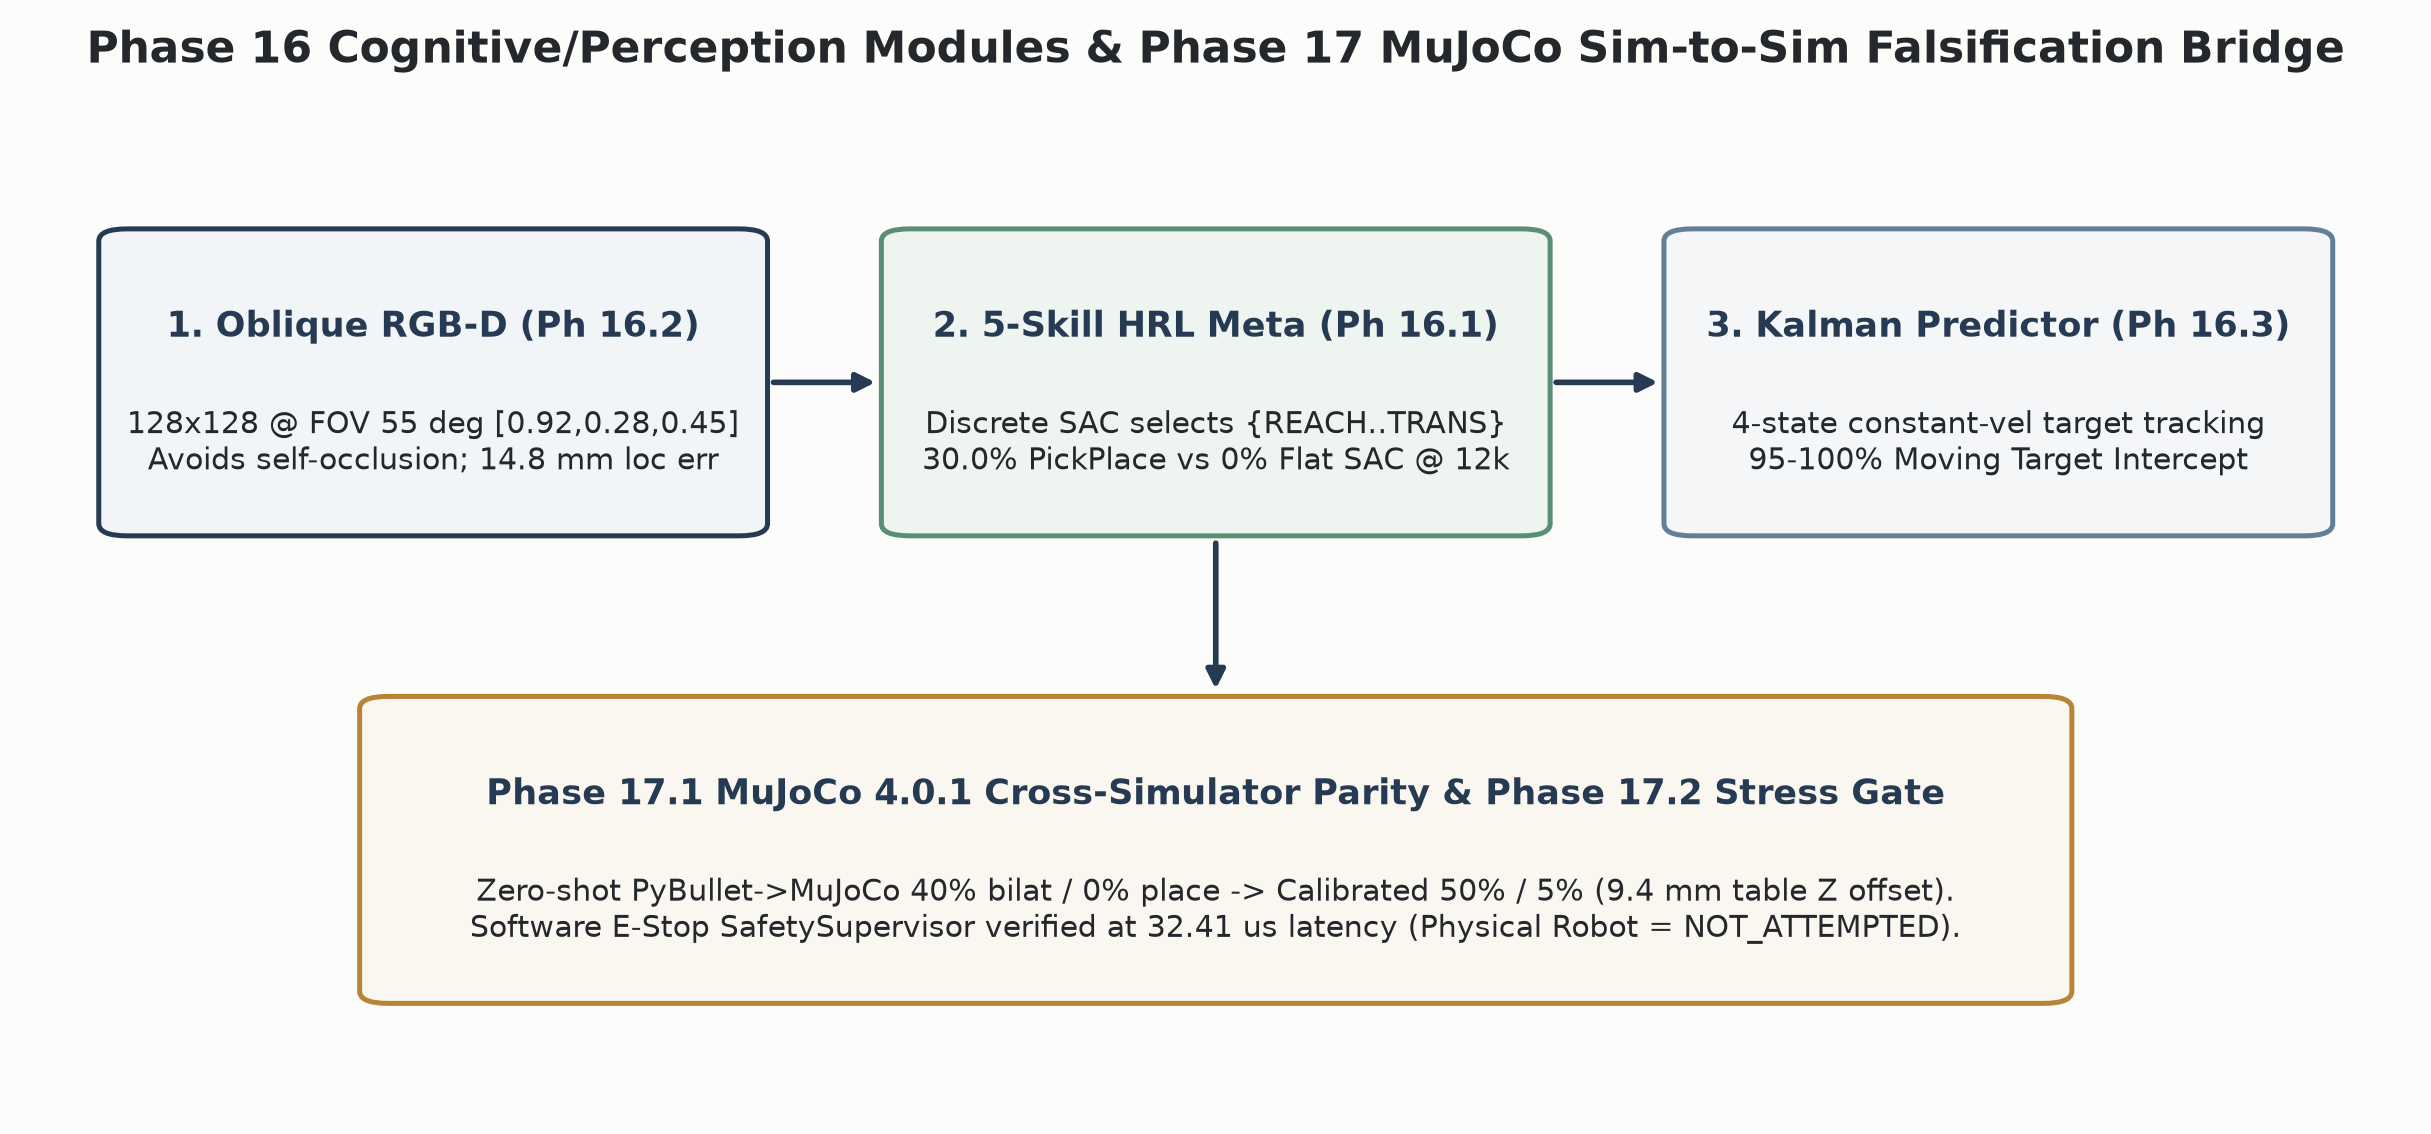
\includegraphics[width=0.9\linewidth]{../../assets/diagrams/diag_11_hrl_rgbd_and_sim2sim.png}\caption{Figure 7.1: Integration across oblique RGB-D perception, 5-skill HRL selection, Kalman dynamic prediction, and MuJoCo validation.}\end{figure}
\begin{figure}[htbp]\centering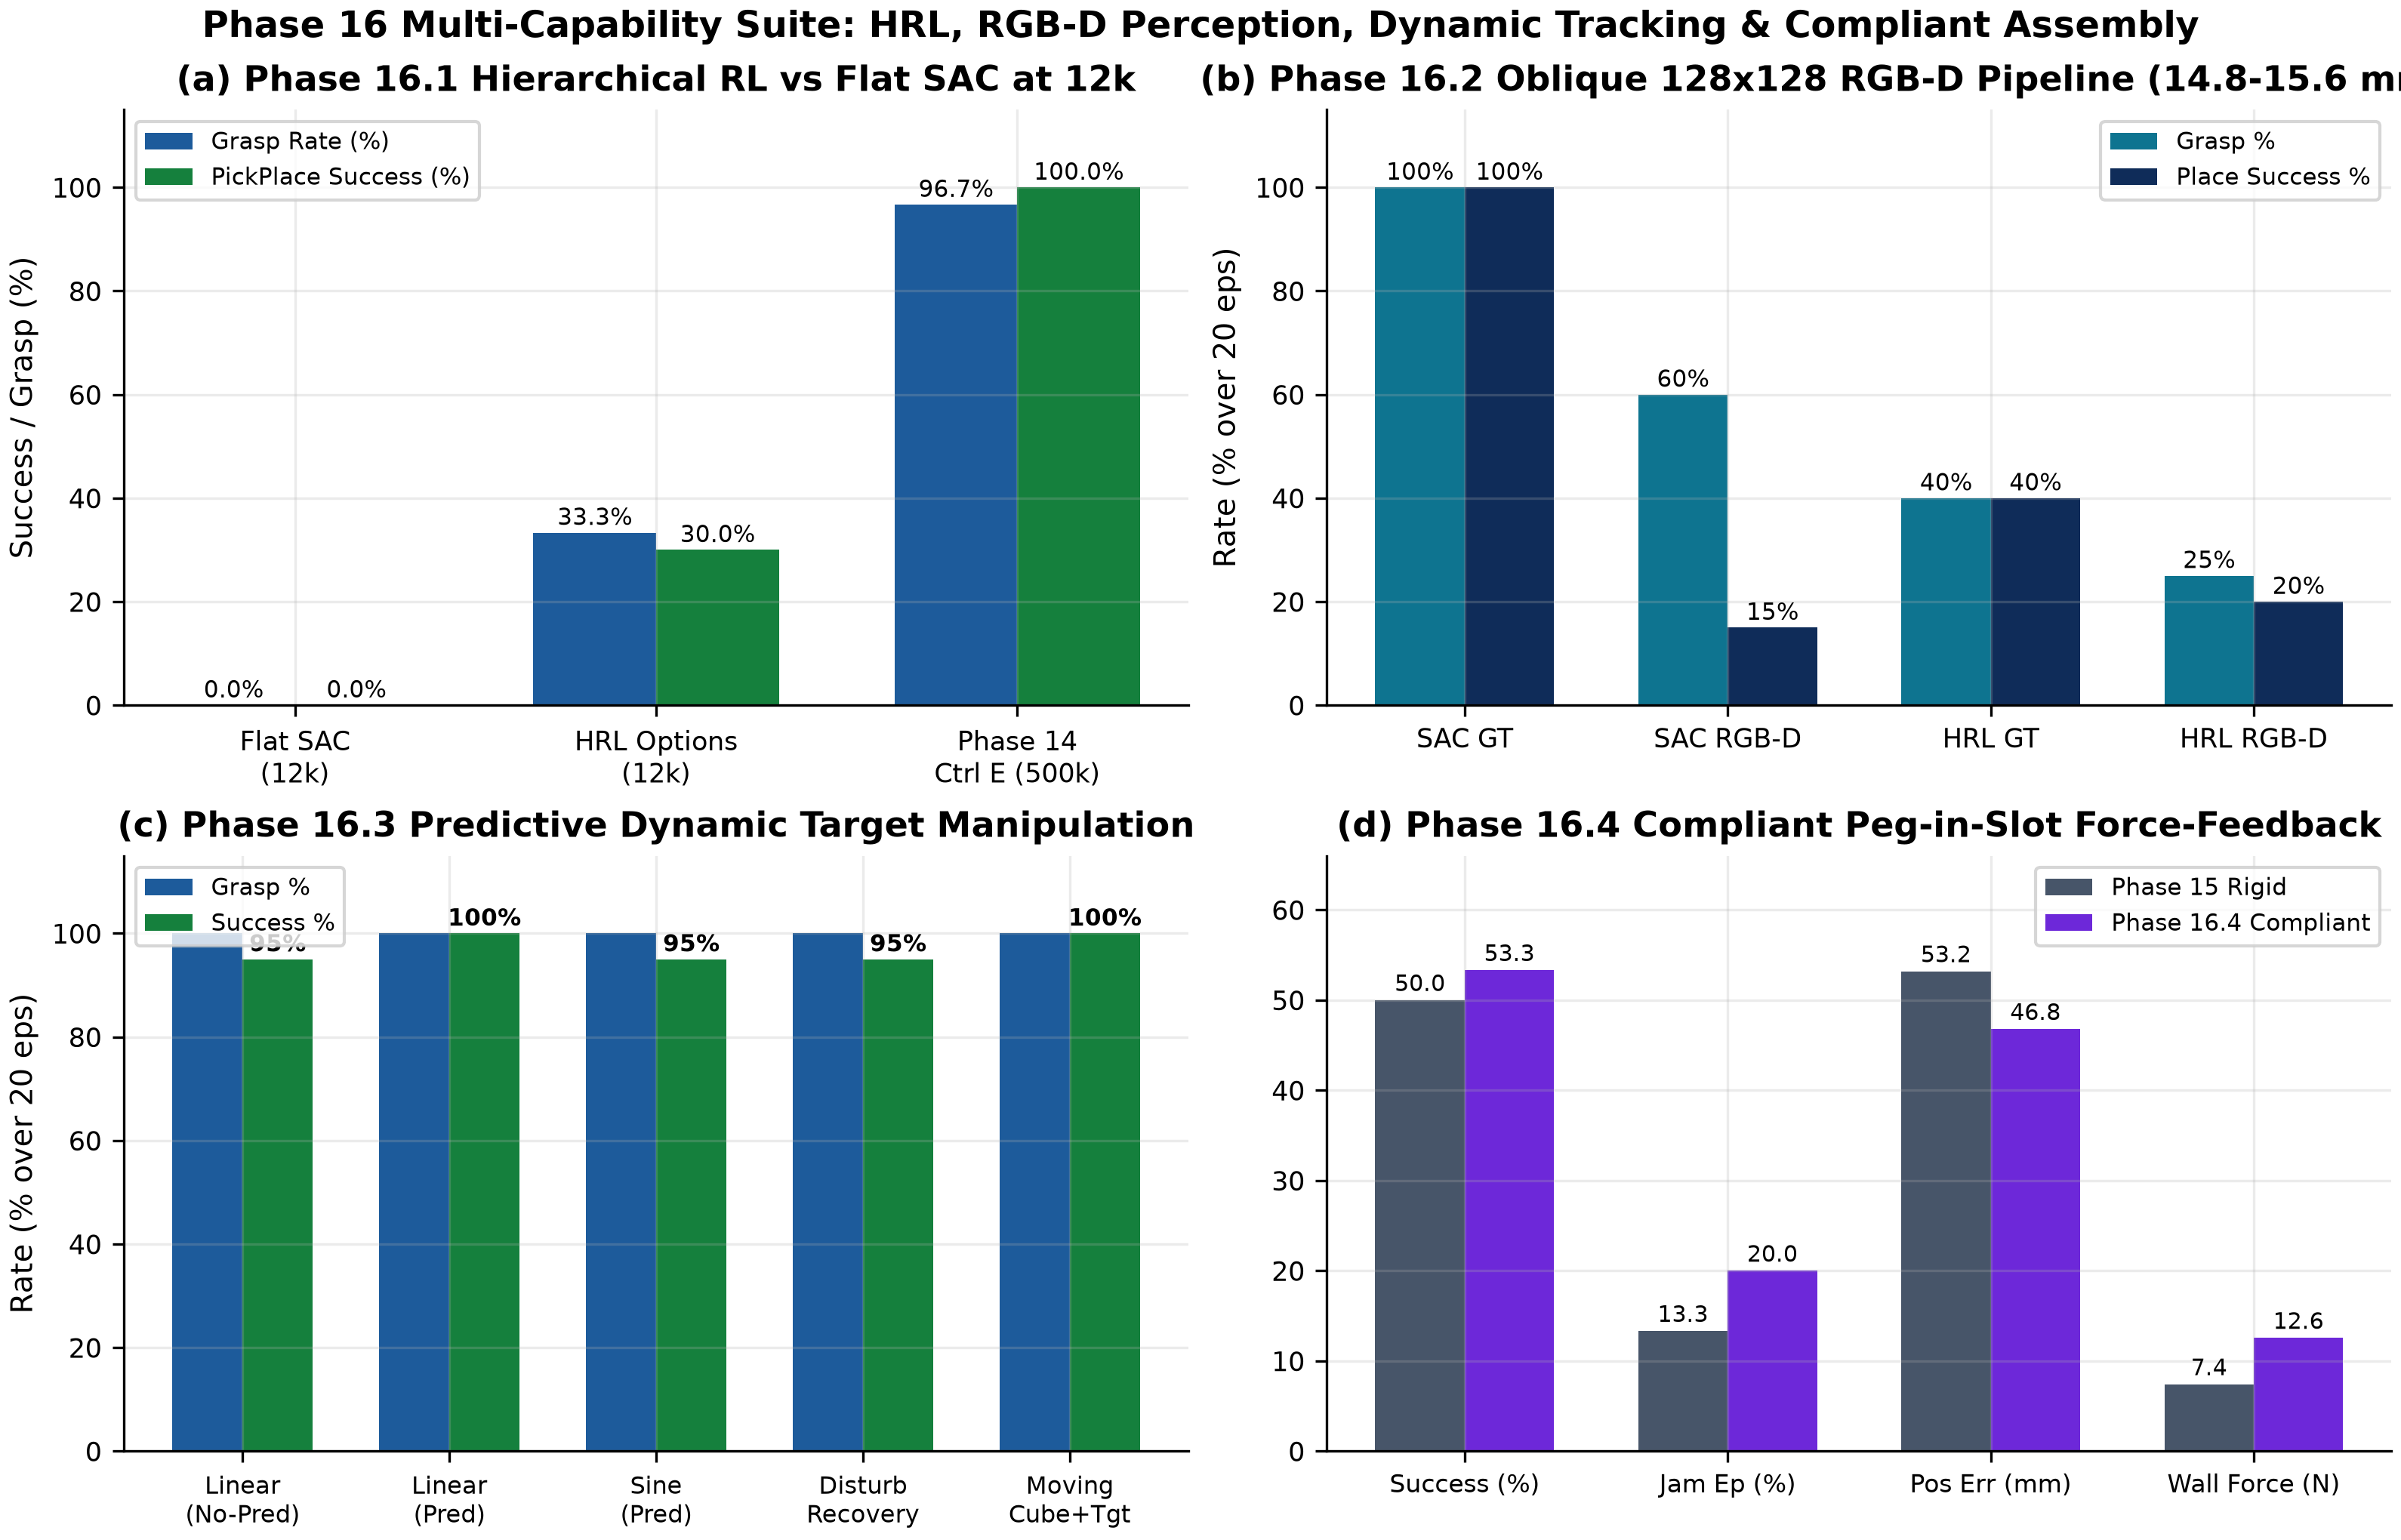
\includegraphics[width=0.9\linewidth]{../../assets/plots/plot_08_phase16_hrl_vision_dynamic_contact.png}\caption{Figure 7.2: Empirical Phase 16 suite across HRL (12k), RGB-D Vision (20 ep), Dynamic Kalman (20 ep/cond), and Compliant Assembly (30 ep).}\end{figure}
\begin{figure}[htbp]\centering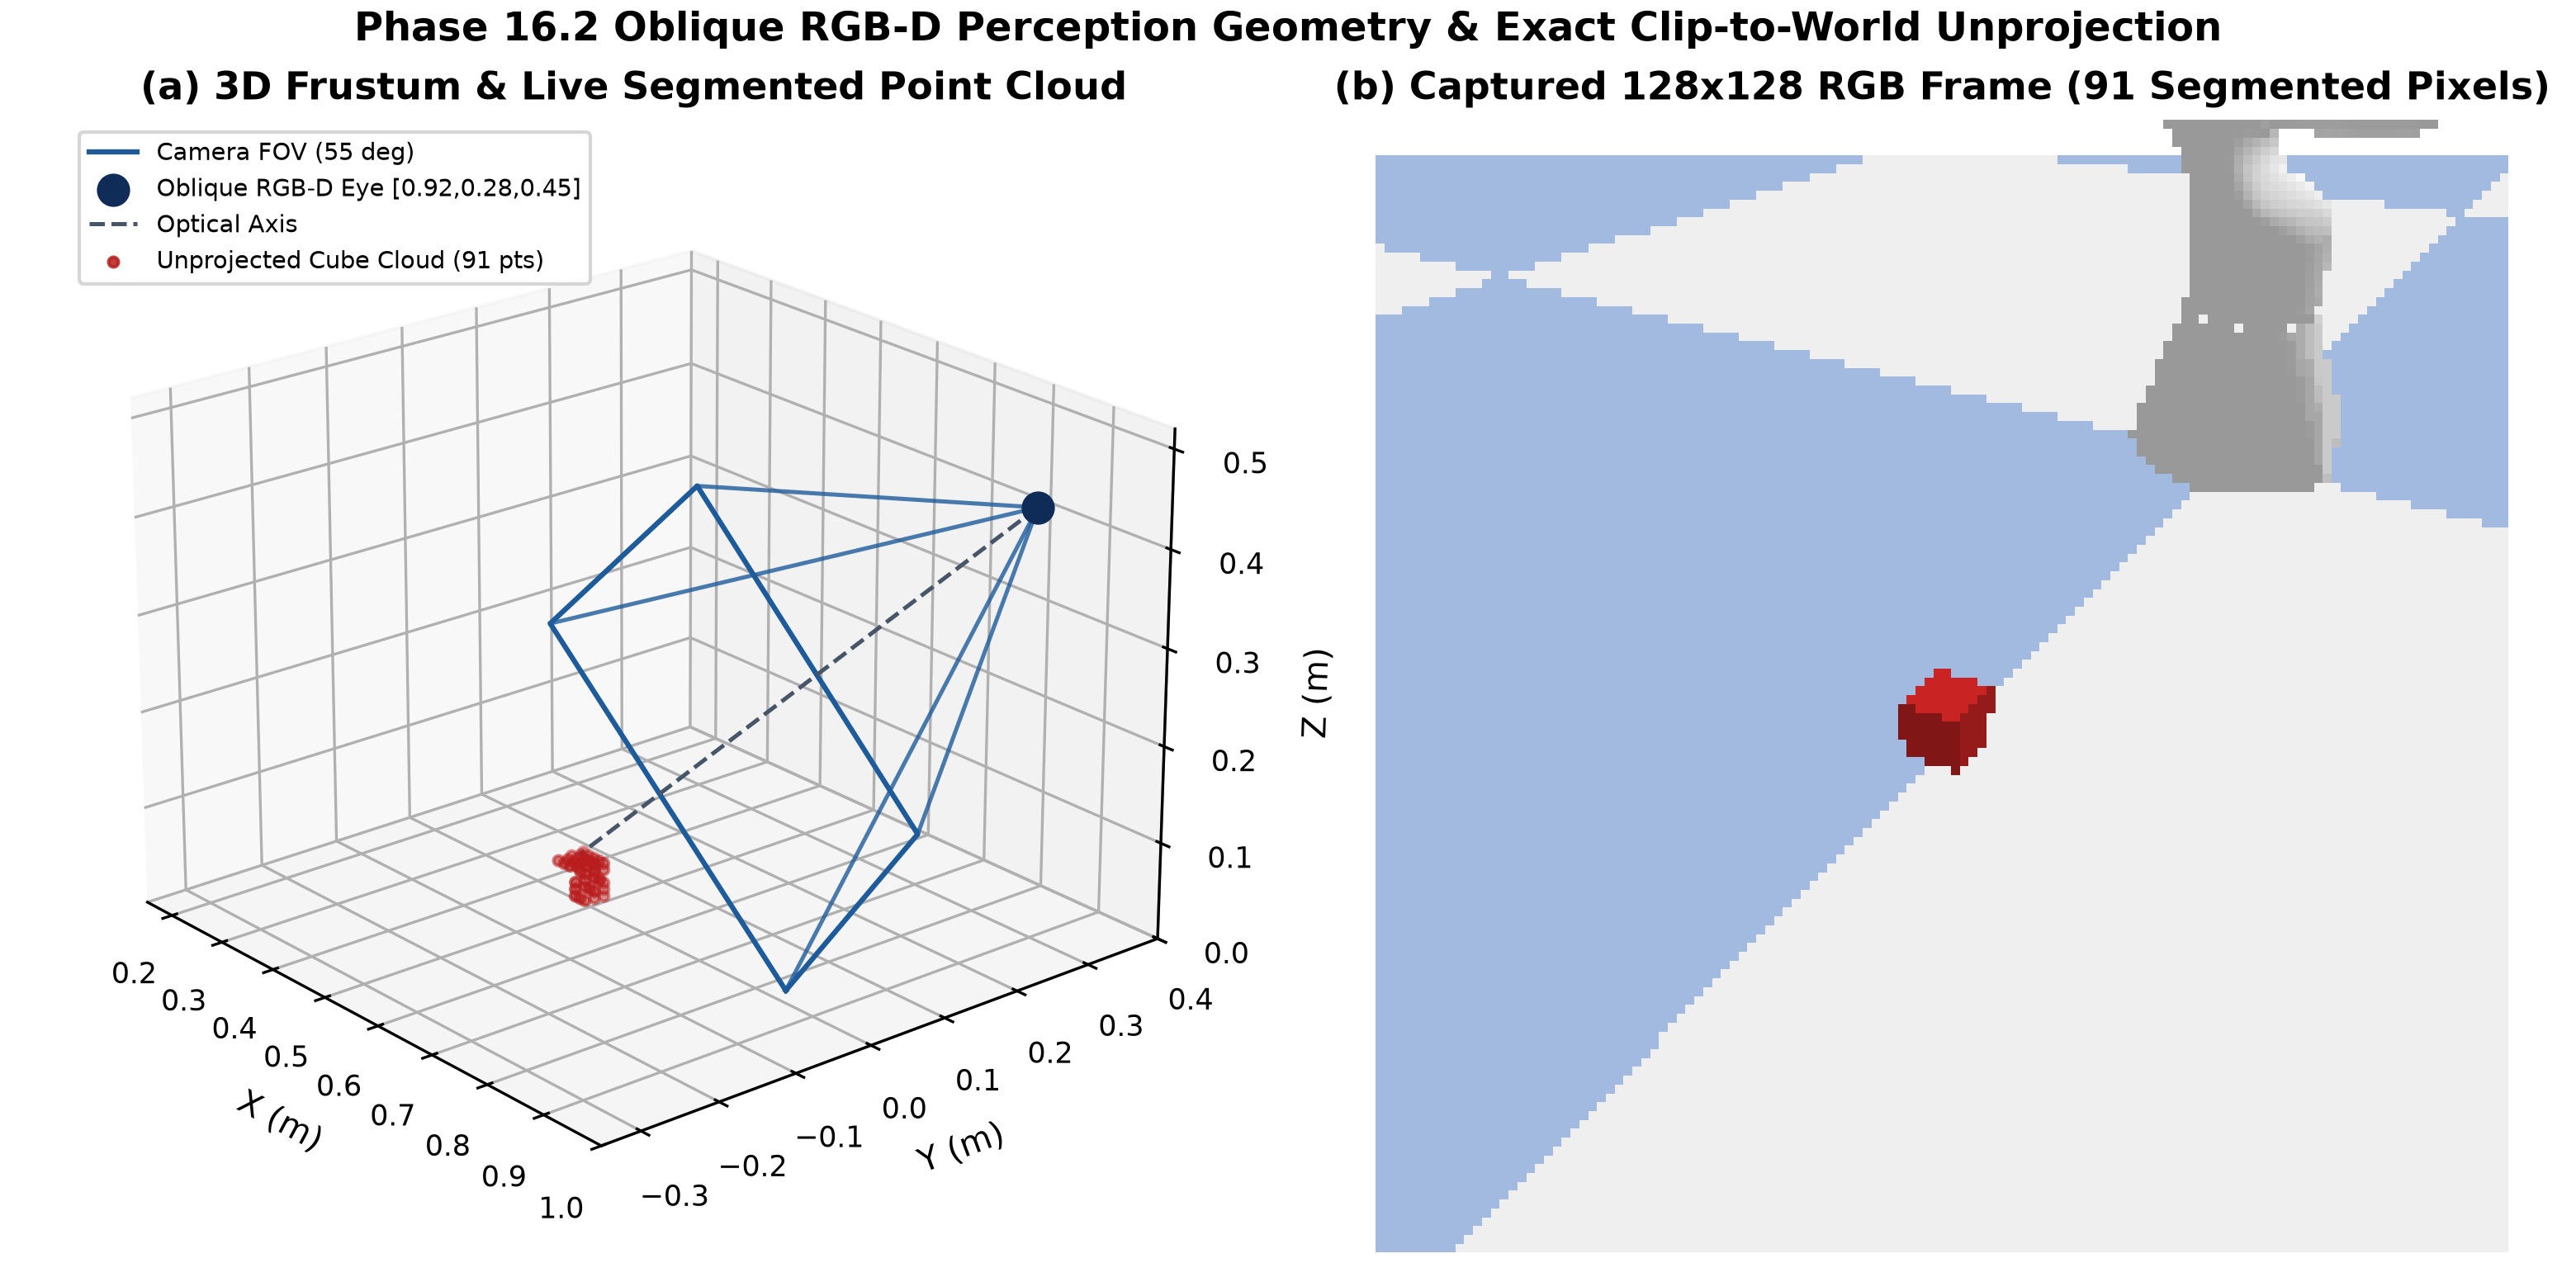
\includegraphics[width=0.9\linewidth]{../../assets/plots/plot_11_oblique_rgbd_3d_frustum.png}\caption{Figure 7.3: Live PyBullet 3D oblique camera frustum (FOV 55 deg) and unprojected 91-pixel cube point cloud.}\end{figure}
\section{7.2 Phase 17: Cross-Simulator Falsification in MuJoCo 4.0.1 \& Deployment Safety}
Porting PickPlace identically into MuJoCo 4.0.1 (`MuJoCoPandaPickPlaceEnv`, Phase 17.1 `PARTIALLY\_COMPLETE` as cross-sim diagnostic) exposed genuine physics-solver differences (`ERR-012` massless MJCF links repaired + 9.4 mm tabletop rest Z offset): frozen PyBullet Seed 42 dropped from 98\% Held-Out DR4 to 40\% bilateral contact / 5\% grasp / 0\% completion zero-shot, improving to 50\% contact / 15\% grasp / 5\% completion after actuator friction/force calibration (Figure 7.4a). Phase 17.2 (`COMPLETE`) validated `SafetySupervisor` runtime E-stop latency at 32.41 us across 250 faulty injections and 100\% stress completion under ±5 mm noise and frequency jitter (Figure 7.4b). Phase 17.3 physical robot execution was explicitly NOT\_ATTEMPTED.

\begin{figure}[htbp]\centering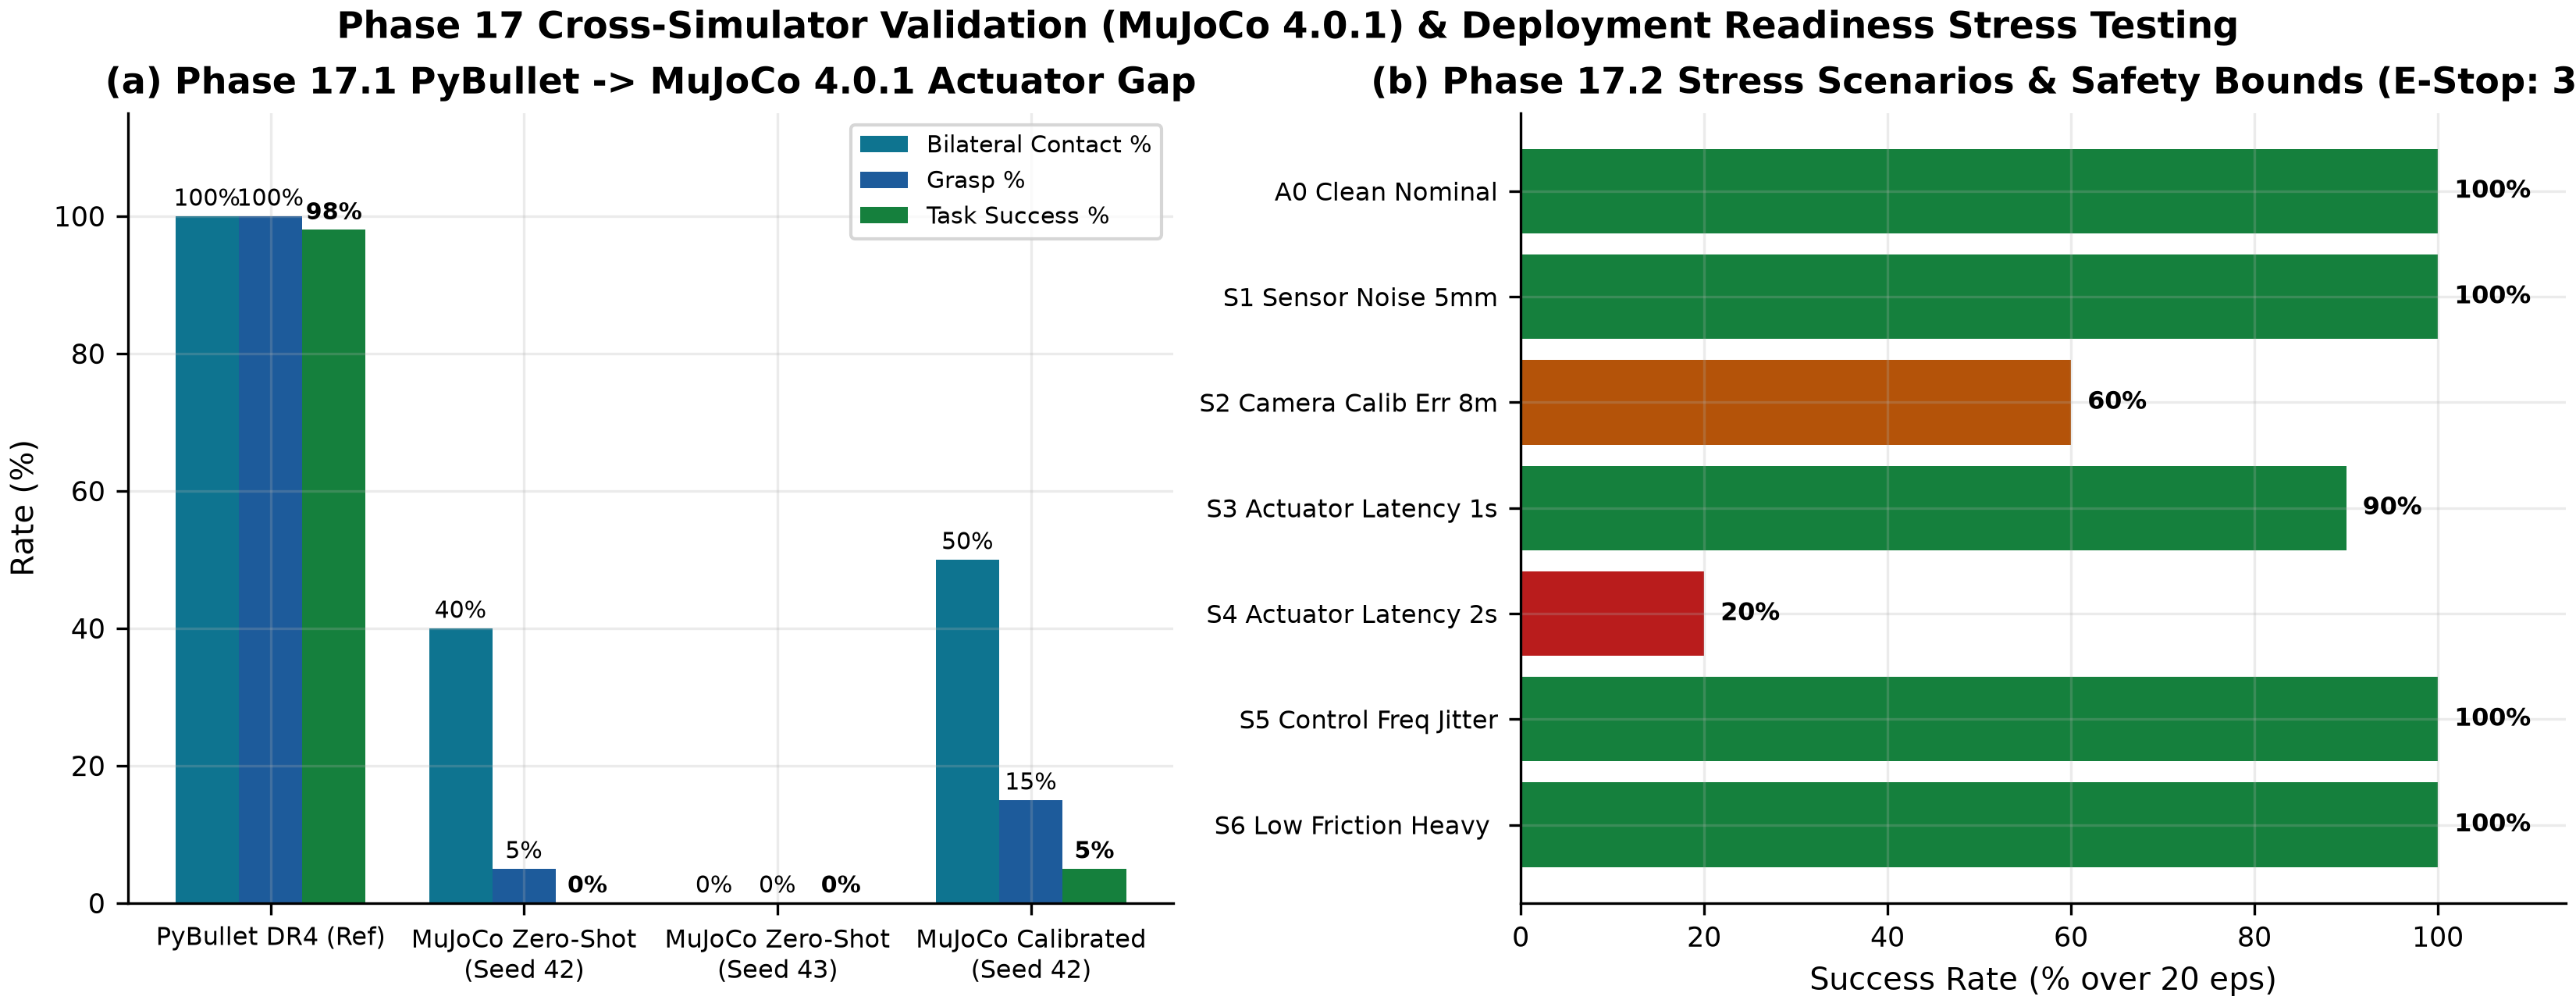
\includegraphics[width=0.9\linewidth]{../../assets/plots/plot_09_phase17_sim2sim_and_safety.png}\caption{Figure 7.4: Phase 17.1 PyBullet-to-MuJoCo 4.0.1 transfer gap and Phase 17.2 simulated stress \& E-stop assessment.}\end{figure}